% codigoFuenteLibroR2
% Copyright (C) 2020  J.M. Perez Zerpa, et. al.
%
% This program is free software: you can redistribute it and/or modify
% it under the terms of the GNU General Public License as published by
% the Free Software Foundation version 3 of the License.
%
% This program is distributed in the hope that it will be useful,
% but WITHOUT ANY WARRANTY; without even the implied warranty of
% MERCHANTABILITY or FITNESS FOR A PARTICULAR PURPOSE. See the
% GNU General Public License for more details.
%
% You should have received a copy of the GNU General Public License
% along with this program.  If not, see <http://www.gnu.org/licenses/>.
%

\chapter[Introducción]{Introducción}

En esta unidad se presentan definiciones y conceptos básicos a ser utilizados en unidades posteriores. %
%
Algunos conceptos fueron vistos en cursos anteriores y otros son introducidos aquí. %
%
Se presentan criterios de clasificación de estructuras y definiciones de análisis y modelado estructural, para lo cual se tomó como referencia parcial el libro publicado por \cite{Hibbeler2012}. %
%
Se repasa el desarrollo de las principales ecuaciones de la teoría de vigas como lo hace \cite{Timoshenko1940a} y se recuerdan los conceptos más importantes de la teoría de Elasticidad Lineal, tomando como referencia los materiales de la Unidad Curricular dictada por \cite{CanelasElasticidad}. %
%
Finalmente se presenta, brevemente, la aplicación del principio de trabajos virtuales al desarrollo de las ecuaciones de elementos estructurales, en particular para el elemento de barra.
%

\section{Análisis y modelado estructural}

% historia
Las estructuras construidas y diseñadas por el ser humano han sido utilizadas, desde la época de los imperios egipcio, romano y griego, para cumplir con diversos tipos de objetivos. %
%
En el renacimiento, entre los siglos XV y XVI, Da Vinci y Galileo comienzan a resolver problemas de estática de barras, poleas y vigas aplicando herramientas matemáticas y conceptos similares a los del principio de desplazamientos virtuales. %
%
Posteriormente entre los siglos XVII y XIX surgieron otros líderes científicos como Hooke, Euler, Bernoulli y Navier, quienes desarrollaron los métodos analíticos de análisis de estructuras de barras en las hipótesis que abordaremos en el curso. %
%
El estudiante interesado puede profundizar en la historia del análisis de estructuras en \citep{Timoshenko1953}. %

En el siglo XX fueron desarrollados métodos prácticos útiles para el análisis de estructuras de gran tamaño como el Método de los Elementos Finitos (MEF) \citep{Zienkiewicz1972}. %
%
En el siglo XXI las herramientas de análisis numérico de estructuras están totalmente integradas al proceso de diseño a través de diversas herramientas. Un ejemplo de esto se ve en el paradigma BIM (\emph{Building information modeling}) y sus formatos correspondientes (como el formato abierto IFC). 

Por último se debe indicar que el desarrollo de métodos numéricos para análisis estructural sigue siendo un área de activa investigación, integrando nuevos enfoques desde otras disciplinas, con el objetivo de lograr análisis más precisos y de forma más eficientes \citep{forets}
% -----------------------------


\subsection{Definición y clasificación de estructuras}

% 
Para poder utilizar un lenguaje común al referirse a las estructuras es necesario y útil establecer definiciones y criterios de clasificación de estructuras. %
%
En el curso se considerará la siguiente definición de \textit{estructura}.

\cajaconcepto{Definición: Estructura}
{Una estructura es un \textbf{sistema de componentes} o elementos estructurales, utilizado para soportar un conjunto de \textbf{cargas} con el objetivo de cumplir una \textbf{función}.}

A continuación se presentan algunos posibles criterios de clasificación de estructuras según su función, cargas y componentes estructurales. %
%


\subsubsection{Clasificación según su función}

Una estructura puede ser clasificada de acuerdo a su función, o la disciplina en la que se presenta, de la siguiente forma:
%
\begin{itemize}
  %
  \item \textbf{Civiles}: estructuras destinadas a cumplir funciones vinculadas a la población civil (como vivienda, comercial o industrial). %
  %
  Los elementos que componen estas estructuras cuentan con geometrías diseñadas de manera óptima para soportar cada tipo de carga, así como también están limitados por los materiales y métodos constructivos disponibles. %
  %
  Las cargas principales consideradas son: peso propio, sobrecarga de uso y viento. Ejemplos: universidades, carreteras, puentes, sistemas de transmisión de energía eléctrica, vías férreas (ver Figura~\ref{fig:viacorc}), muelles, etc.
  %
  \item \textbf{Mecánicas}: estructuras vinculadas a máquinas o algún componente de equipamientos mecánicos. Presentan gran diversidad de geometrías y tipos de cargas. Ejemplos: estructuras de automóviles (carrocería, motores, etc.), atracciones mecánicas (ver Figura~\ref{fig:barco}).
  %
  \item \textbf{Aeroespaciales}: estructuras de vehículos aeroespaciales. Las cargas suelen estar vinculadas a condiciones extremas o exigentes como altas presiones o temperaturas, o cargas repetitivas que producen fatiga. Ejemplos: aviones, satélites \citep{Yoshiaki1992}.
  %
  \item \textbf{Navales}: estructuras vinculadas a actividades navales, como por ejemplo, componentes de barcos. Las cargas tienen una componente dinámica importante, así como también una complejidad elevada debido a la interacción con fluidos.
  %
  \item \textbf{Biomédicas}: estructuras de soporte de componentes biomédicos. Eventualmente sometidas a procesos químicos. Ejemplos: prótesis, \textit{stents} \citep{Frischkorn2015}.
  %
\end{itemize}

% ---------------------------------
\begin{figure}[htb]
	\centering
\subfloat[Ejemplo de estructura civil: vía férrea de tren de Corcovado en Río de Janeiro, Brasil.]{
	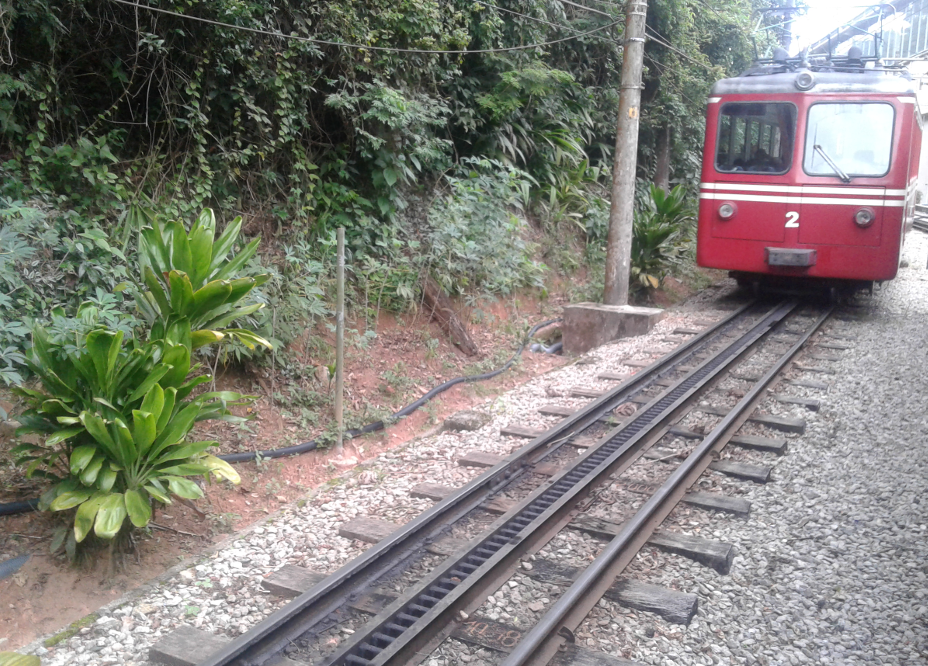
\includegraphics[width=0.48\textwidth]{viacorc}
	\label{fig:viacorc}	
}
%\hspace{0.01\textwidth}
~
\subfloat[Ejemplo de estructura mecánica: atracción mecánica en Montevideo, Uruguay.]{
	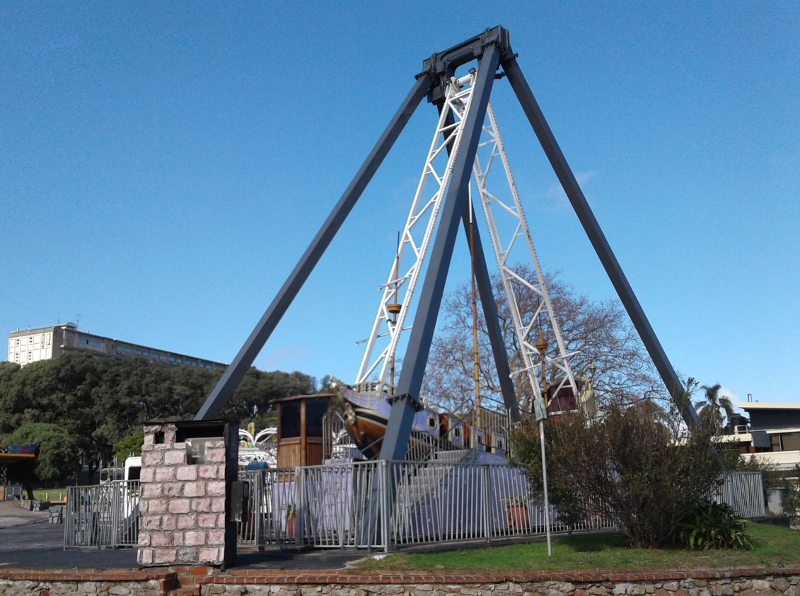
\includegraphics[width=0.47\textwidth]{barcopirata}
	\label{fig:barco}	
}
\caption{Ejemplos de estructuras.}
	\label{fig:ejsestr}
\end{figure}
% ---------------------------------

En este texto se presentan métodos de análisis aplicables principalmente a \underline{estructuras civiles}.









\subsubsection{Clasificación de componentes estructurales}

Las estructuras civiles están formadas por \textit{componentes estructurales}, los cuales son descritos de forma sintética a continuación:
%
\begin{itemize}
	\item \textbf{barra}: elemento con una dimensión (eje) considerablemente mayor que las otras. Soporta tensiones de compresión o tracción según su eje.
	%
	\item \textbf{viga } (de eje recto): elemento con geometría de barra en su configuración natural (sin cargas), que puede ser sometido a fuerzas según su eje (normales) o transversales (cortantes) así como también a momentos según su eje (torsores) o transversales (flectores).
	%
	\item \textbf{pilar}: elemento con geometría de barra que se encuentra sometido a flexión y compresión según su eje, siendo la compresión preponderante.
	%
	\item \textbf{cable}: también utilizado como \textbf{tensor}, son elementos de barra sometidos principalmente a tracción que no soportan considerable flexión o compresión según su eje.
	%
	\item \textbf{losa y cáscara}: elementos con una geometría tal que una dimensión es considerablemente menor que las otras dos. La dimensión menor define el espesor, mientras que las otras dos definen el plano medio (o superficie media) de la losa (o cáscara). %
	%
	Soportan flexión o tensión con vector contenido en el plano medio. %
	%
	Las losas tienen un plano medio plano, mientras que en las cáscaras, este se encuentra dado por una superficie con curvatura no nula.
	%
	\item \textbf{membrana}: elementos superficiales muy flexibles de pequeño espesor que no son capaces de soportar compresión o flexión. %
	%
	En la Figura~\ref{fig:termmadero} se observa la cubierta exterior, de la Terminal Madero de la Ciudad de Buenos Aires, formada y soportada por componentes de membrana, barras, vigas y cables.
	%
	\item \textbf{otros}: existen otros elementos estructurales con geometrías más complejas no asociados directamente a un estado tensional como los anteriores. Algunos ejemplos de estas estructuras son: zapatas, cabezales, muros de contención (trabajando como losa o bajo estados planos de deformación) y arcos, o vigas de eje curvo.
\end{itemize}

\begin{figure}[htb]
	\centering
	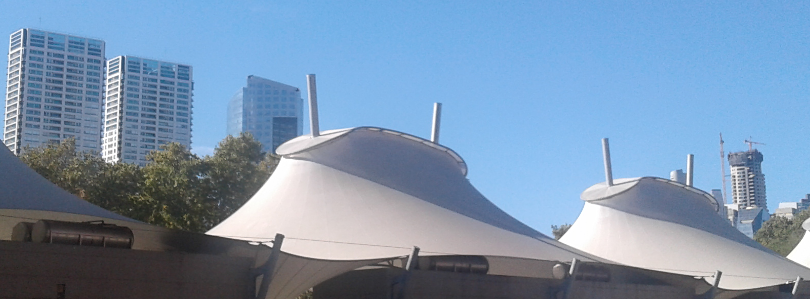
\includegraphics[width=.95\textwidth]{terminalmaderoB}
  \caption{Foto exterior de las cubiertas de la Terminal Madero Ciudad de Buenos Aires, Argentina.}
\label{fig:termmadero}
\end{figure}

Un tipo de estructura frecuentemente analizada es el pórtico, o estructura aporticada, la cual está formada por pilares y vigas vinculados por al menos un nudo rígido o uniones que transmiten momentos. %
%
A continuación se presentan criterios de clasificación de estructuras de acuerdo a los vínculos existentes entre sus componentes.




\subsubsection{Clasificación según sus vínculos}

Se considerarán dos tipos de estructuras de acuerdo a sus vínculos internos:
%
\begin{itemize}
\item \textbf{Estructura reticulada}: formada por barras unidas de forma tal que no se transmiten momentos en todos los nodos de la estructura, es decir que todos los nodos son articulaciones.
%
\item \textbf{Estructura aporticada}: formada por barras unidas donde al menos dos barras están conectadas por un nudo rígido o un vínculo que transmite momentos.
\end{itemize}




\subsubsection{Clasificación según geometría y carga} \label{sec:clasifest}

De acuerdo a su geometría y cargas aplicadas una estructura puede ser clasificada de la siguiente forma.
%
\begin{itemize}
  \item \textbf{Estructura Plana}: Una estructura será considerada \textbf{plana} si se cumplen todas las siguientes condiciones:
    \begin{enumerate}
       \item todos los ejes de sus barras (barras, vigas o pilares) pertenecen a un plano y este plano es plano de simetría de todas las barras de la estructura
       %
       \item todos los vectores de fuerza aplicados a la estructura son vectores contenidos en el plano de simetría de la estructura
       %
       \item todos los momentos aplicados son aplicados en puntos que pertenecen al plano medio de la estructura y están dados por un vector perpendicular al plano de simetría de la estructura
       %
       \item las restricciones cinemáticas son tales que las reacciones correspondientes cumplan con las condiciones anteriores de fuerza y momento.
    \end{enumerate}
  %
  \item \textbf{Estructura Plano-espacial}: Una estructura será considerada \textbf{plano-espacial}, también llamada emparrillado, si se cumple: 
    \begin{enumerate}
	\item todos los ejes de sus barras pertenecen a un plano,
	%
	\item todos los vectores de fuerza aplicados a la estructura son vectores perpendiculares a dicho plano
	%
	\item todos los momentos aplicados son aplicados en puntos que pertenecen al plano de las barras de la estructura y están dados por vectores contenidos en dicho plano
	%
	\item las restricciones cinemáticas son tales que las reacciones correspondientes cumplan con las condiciones anteriores de fuerza y momento.
\end{enumerate}
  
  \item \textbf{Estructura tridimensional}: una estructura será considerada \textbf{tridimensional} si no es clasificada dentro de ninguna de las dos categorías anteriores.
\end{itemize}

\cajaactividad{
	Considere un edificio de viviendas de tres pisos de altura con planta rectangular. %
	%
	Identificar los componentes estructurales de la estructura. %
	%
	Clasifique la estructura de acuerdo a los criterios vistos.}






\subsection{Análisis de estructuras}

Luego de haber definido el término \textit{estructura} se pasa a introducir el concepto de \textit{análisis estructural}. %
%
El análisis es una etapa crucial en el proceso de diseño y verificación de cualquier estructura.

\cajaconcepto{Definición: Análisis estructural}
{El \textit{análisis} de una estructura consiste en la determinación de los \textbf{efectos} (solicitaciones y movimientos) que un sistema de \textbf{cargas} dado produce sobre la \textbf{estructura} y cada uno de los elementos estructurales que la componen.}

El proceso de analizar una estructura y obtener todas las solicitaciones de sus elementos estructurales, es usualmente llamado \textit{resolver} una estructura. %

Las fuerzas aplicadas a los elementos estructurales y la vinculación existente entre estos elementos determinan las deformaciones y solicitaciones de la estructura. %
%
Para definir el tipo de análisis a realizar se deberá categorizar las cargas y vínculos entre componentes. %

A continuación se definen distintos tipos de \textbf{cargas} que suelen ser aplicados a estructuras. Luego se enumeran algunos de los vínculos entre componentes estructurales más importantes.

\subsubsection{Cargas}

Las cargas o fuerzas externas que pueden ser aplicadas a estructuras pueden tener diversas causas, por lo que tendrán diferentes características respecto a: frecuencia de ocurrencia, magnitudes, confiabilidad, etc. Las normas o códigos establecen metodologías para considerar la distinta naturaleza de las acciones al diseñar estructuras.

En este material se considera que toda carga es de tipo \textit{estática} o \textit{permanente}, independientemente de su origen. %
%
Estas cargas son provocadas por acciones cuya magnitud o sentido no varía en el tiempo, como por ejemplo el peso propio de cada elemento estructural. %

Las cargas o esfuerzos producidos por otras acciones como viento, sismos, impactos, etc., deben ser analizadas de forma diferente aplicando modelos numéricos o criterios de diseño específicos definidos por normativas correspondientes. Como ejemplo, se puede ver la  forma en que se definen cargas en la norma europea\footnote{Eurocódigo 1: UNE-EN 1991-1-2:2019 \href{https://www.une.org/encuentra-tu-norma/busca-tu-norma/norma?c=N0061459}{https://www.une.org/encuentra-tu-norma/busca-tu-norma/norma?c=N0061459}}.

En este texto se asume que, sea cual fuere su origen, toda carga podrá ser considerada como estática. %
%
Existe una importante rama de la Ingeniería Estructural, enfocada al análisis dinámico de estructuras, en la cual se destacan referencias bibliográficas como \citep{clough1993dynamics}.
%
% ------------------------


\subsubsection{Condiciones de vínculo y apoyo en estructuras}

Los \textit{vínculos a tierra}, o condiciones de apoyo, de cada nodo de una estructura pueden ser clasificados de la siguiente forma:
%
\begin{itemize}
\item \textbf{libre}: un nodo o un extremo de una viga que no está vinculado a tierra o que no tiene desplazamiento ni giro impuesto ni restringido en ninguna dirección o ángulo,
%
\item \textbf{desplazamiento impedido}: vínculo que impide el desplazamiento de un nodo en una o más direcciones,
%
\item \textbf{giro impedido}: vínculo que impide el giro de un nodo según un cierto vector,
%
\item \textbf{resorte de desplazamiento}: vínculo en el cual la fuerza externa aplicada es proporcional y de sentido contrario al desplazamiento desarrollado por el nodo en una cierta dirección,
%
\item \textbf{resorte de giro}: vínculo en el cual el momento externo aplicado es proporcional y de sentido contrario al giro desarrollado por el nodo en una cierta dirección,
%
\item \textbf{vínculo mixto}: vínculo con combinaciones que no pertenecen a ninguna de las categorías anteriores.
%
\end{itemize}

En la Figura~\ref{fig:membr} se muestra parte de la estructura de soporte de la cubierta de la terminal de Madero en Buenos Aires. %
%
En la Figura~\ref{fig:artic} se puede ver una materialización de un vínculo que podría considerarse como un apoyo fijo que restringe el desplazamiento de un punto. %
%
El modelado estructural de este vínculo puede ser un problema interesante, donde es necesario estudiar el nivel de restricción real del giro en algunas direcciones. %
%
\begin{figure}[htb]
	\centering
	\subfloat[Elementos de transmisión de cargas y soporte.]{
	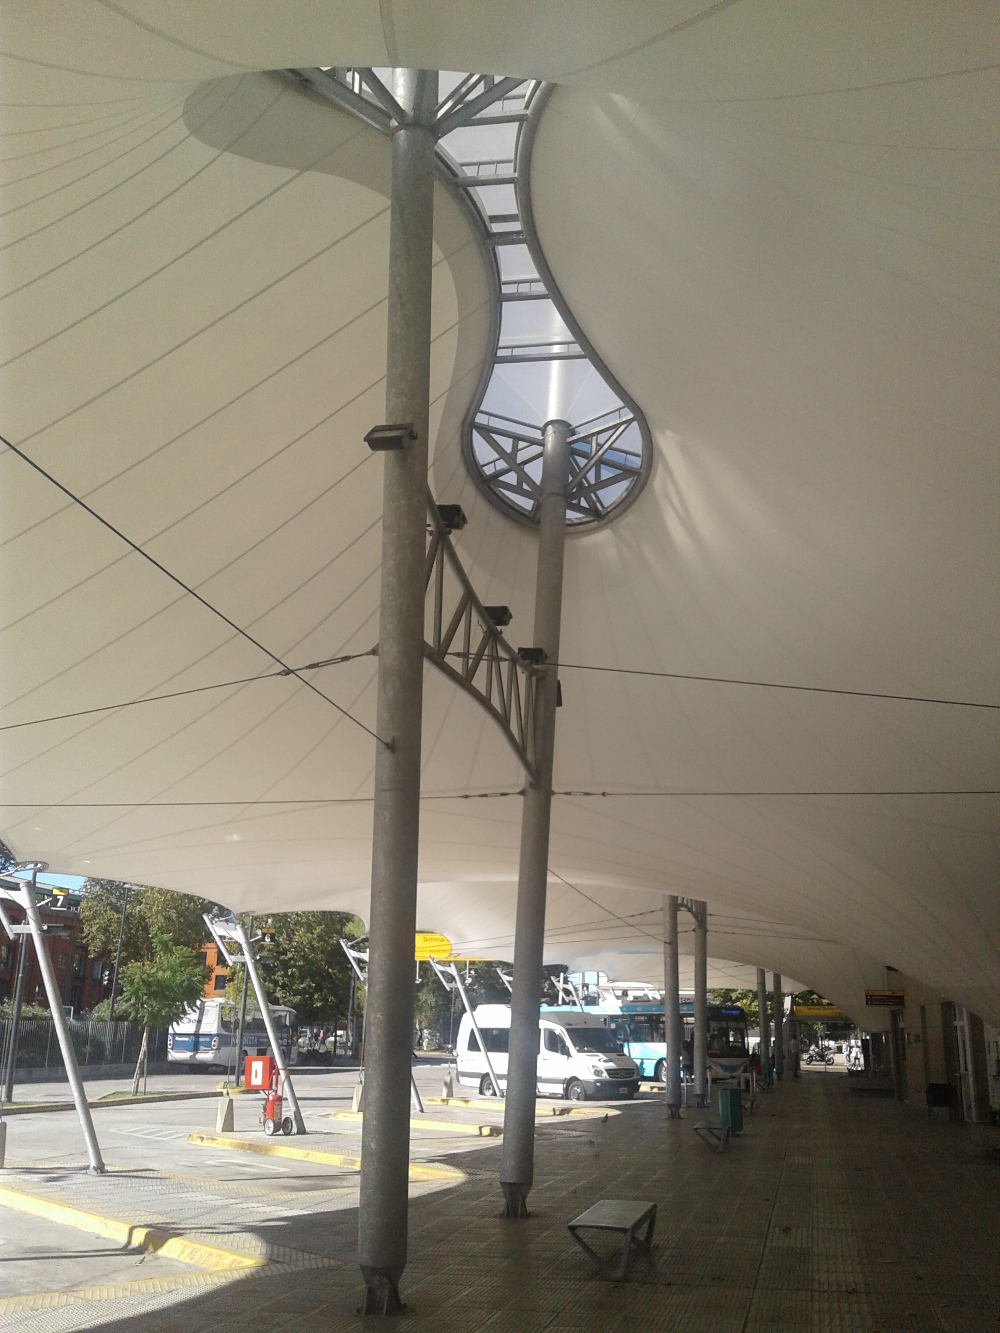
\includegraphics[width=0.38\textwidth]{membranal}
	\label{fig:membr}
}
	\subfloat[Elementos de transmisión de cargas y soporte.]{
	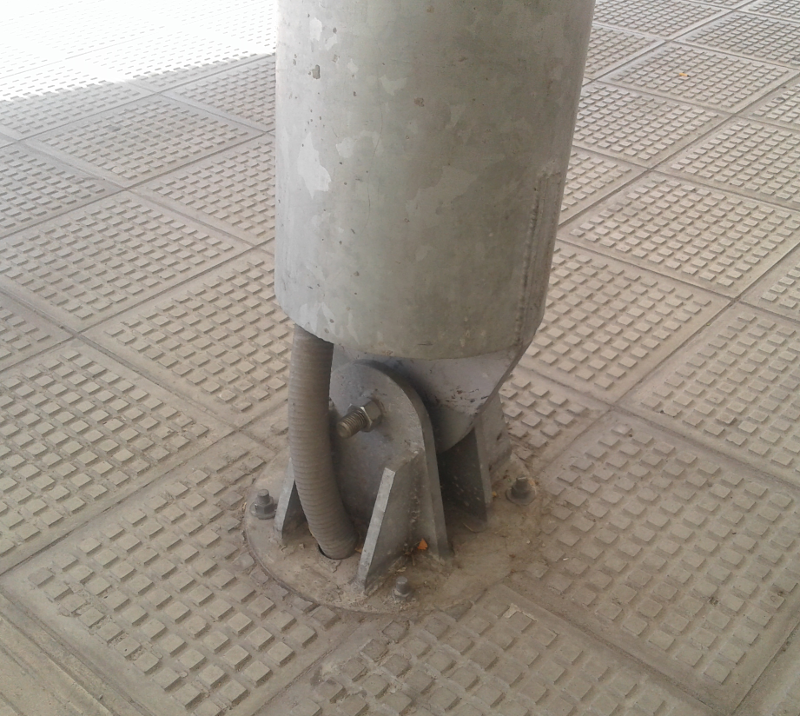
\includegraphics[width=0.57\textwidth]{artic}
	\label{fig:artic}
	}
	\caption{Fotos de interior de terminal Madero, Ciudad de Buenos Aires.  (izq.), vínculo a tierra articulado (der.).}
	\label{fig:bsas}
\end{figure}

\subsubsection{Clasificación de vínculos entre elementos estructurales}

El comportamiento de los elementos estructurales están limitado por los vínculos, que pueden ser clasificados como:
%
\begin{itemize}
\item \textbf{articulación}: nodo que transmite fuerzas y compatibiliza desplazamientos entre barras que llegan a el,
\item \textbf{unión rígida}: nodo que transmite fuerzas y momentos y compatibiliza desplazamientos y giros entre barras que llegan a el,
\end{itemize}

Existen otros tipos de vínculos que pueden ser considerados entre elementos estructurales, pero no serán vistos en el curso.

\cajaactividad{
Enumere las cargas presentes durante la vida útil del edificio de tres pisos considerado en la actividad anterior. %
%
Analice qué tipo de apoyo puede tener la estructura sobre el suelo así como también qué vínculos pueden existir entre los elementos de la estructura.}












\subsection{Modelado estructural}

% presentacion conceptos
El análisis estructural es la herramienta utilizada por profesionales responsables del diseño de estructuras. %
%
El diseño de una estructura consiste en un proceso iterativo en el cual se definen dimensiones de los componentes estructurales, se determinan sus solicitaciones y se verifica que se cumpla con el criterio del profesional y las normativas correspondientes. %
%

Para presentar de forma esquemática el proceso asociado al diseño de una estructura se definen los siguientes conceptos:
%
\begin{itemize}
  \item Estructura Real (ER)
  \item Esquema Básico de Cálculo (EB)
  \item Modelo Numérico (MN)
\end{itemize}
% ---

\paragraph{Estructura Real}
%
El concepto de \textit{Estructura Real} (ER), podrá ser utilizado para referirse a una estructura existente (ya construida), o a aquella que se desea construir y que es imaginada por los diseñadores. %
%
En toda ER se cuenta con una geometría con imperfecciones debidas al procedimiento constructivo. %
Asimismo, la ER está sometida a estados de cargas asociadas al uso efectivo que tiene a lo largo de su vida útil. %
%
Las condiciones de apoyo también son debidas a la interacción de la misma con otros elementos como, por ejemplo, el apoyo sobre un suelo no homogéneo, el cual tiene un comportamiento complejo de alta dificultad para predecir.


\paragraph{Esquema Básico de Cálculo}
%
El \textit{Esquema Básico de cálculo} (EB), es considerado como el modelo simplificado de la estructura que se obtiene al considerar ciertas hipótesis sobre la estructura real. %
%
Como ejemplos se tiene: una geometría idealizada, condiciones de apoyos ideales (por ej. apoyos fijos) o estados de carga hipotéticos, establecidos por normas técnicas y con cierta probabilidad de ocurrencia. %
%
También se pueden incluir aquí las hipótesis sobre el comportamiento constitutivo de los materiales que componen la estructura, frecuentemente estipulado por normas técnicas.

\paragraph{Modelo Numérico}
%
El \textit{Modelo Numérico} (MN) de una estructura es la herramienta que se utiliza para obtener magnitudes solución de las ecuaciones asociadas al EB (es decir, desplazamientos, solicitaciones, tensiones, etc). %
%
Para estas soluciones se debe utilizar algún método numérico para resolver un conjunto de ecuaciones lineales o en algunos casos no lineales \citep{Bazzano2017}. %
%


El proceso de diseño estructural consiste en un procedimiento iterativo que puede ser sintetizado de forma simplificada a través de la siguiente lista de etapas:
%
\begin{enumerate}
  \item establecer \textbf{condiciones} que la ER debe cumplir (arquitectónicas, normativas, etc.)
  %
  \item \textbf{definir un EB} a partir de una primer estimación de secciones, materiales, vínculos entre componentes
  %
  \item a través del uso de un MN \textbf{obtener las solicitaciones} a las que cada componente de la estructura estará sometido
  %
  \item \textbf{diseñar los componentes} de las estructuras para soportar las solicitaciones (acero, secciones, tipo de hormigón, etc.) 
  %
  \item \textbf{verificar} si se cumplen las condiciones definidas en (1): si se cumplen entonces se finalizó, si no se cumplen se debe proponer un nuevo EB recomenzando desde el paso (2).
\end{enumerate}


En este curso se abordará el estudio de métodos analíticos y numéricos para la determinación de solicitaciones y desplazamientos (análisis) de estructuras. %
Esto corresponde a la etapa 3 del proceso de diseño descrito. %
%
En menor medida se realizará diseño de secciones considerando criterios simples de resistencia de materiales sin tomar en cuenta las consideraciones más complejas definidas por las normas técnicas necesarias para el ejercicio profesional. %
%
%A partir de un análisis adecuado del EBCE, el ingeniero decide aspectos como el tipo y cantidad de elementos a utilizar, forma de introducción de los estados de carga y método numérico utilizado para realizar el análisis del problema en función del modelo constitutivo del material.
%

\subsection{Ejemplo: Análisis simplificado de puente metálico}

Para fijar ideas se considera un ejemplo de modelado simple de una estructura compleja. %
%
Con esto, se pretende mostrar parte del proceso de modelado y análisis de una estructura para ilustrar los conceptos introducidos.

En la Figura~\ref{fig:raila} se muestra una foto de un puente metálico, que será considerado como la \textbf{estructura real}. %

\begin{figure}[htb]
  \centering
	\subfloat[Foto de Estructura Real.]{
	  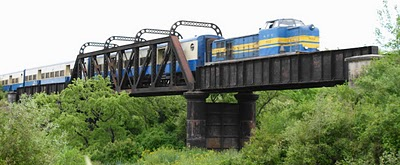
\includegraphics[width=0.7\textwidth]{ferroviario}\label{fig:raila}
    }\\
	\subfloat[Esquema Básico de Cálculo.]{
	  \resizebox{.9\linewidth}{!}{\input{./figs/UT1/reticRail.pdf_tex}}\label{fig:railb}
    }\\
	%
	\subfloat[Diagrama de deformada con factor de escala 10 y escala de colores de tensiones axiales.]%
	{
	  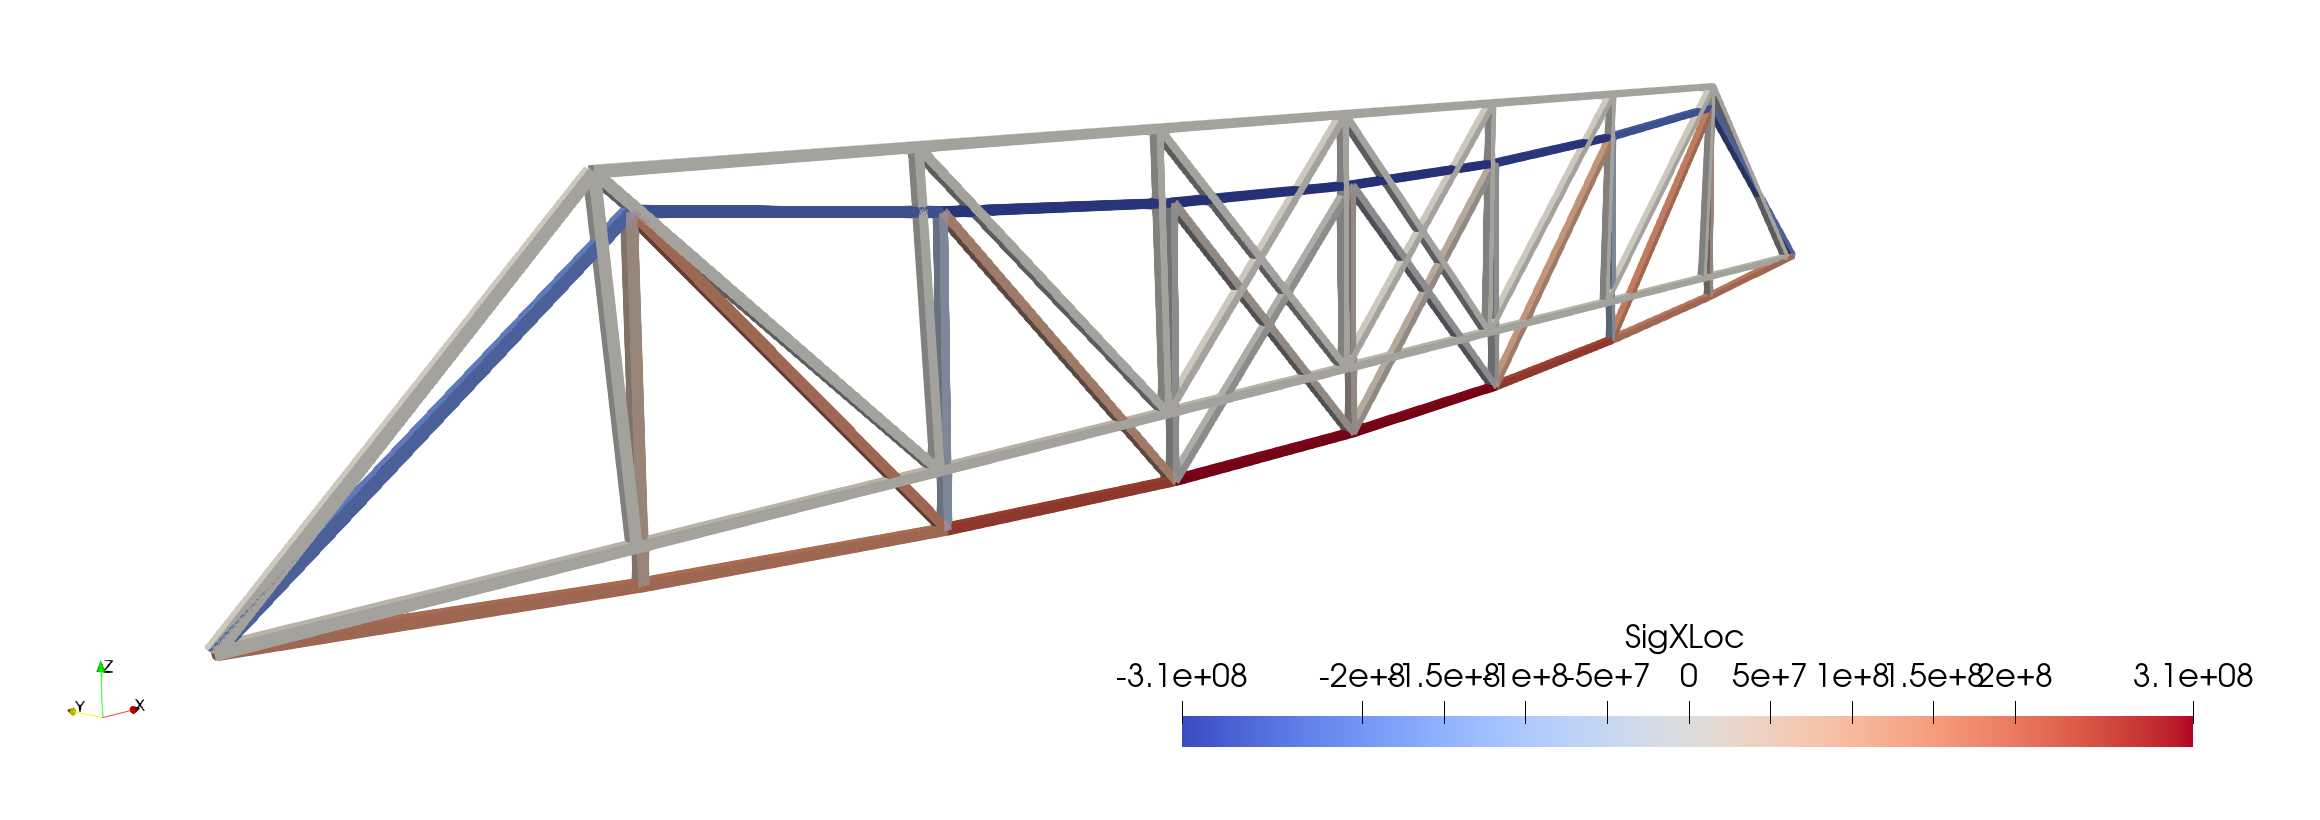
\includegraphics[width=0.9\textwidth]{reticRailDeform}\label{fig:railc}}
  \caption{Ejemplo simplificado de las principales componentes en el proceso de diseño o verificación de una estructura.}
\end{figure} 


Para pasar al EB se consideran diversas hipótesis, entre las que se destacan:
\begin{itemize}
  \item las uniones de los perfiles son consideradas como articulaciones,
  %
  \item las cargas puntuales aplicadas en los nodos se consideran de igual magnitud,
  %
  \item se consideran dos reticulados planos con todos sus nodos desplazandose en el plano que los contiene, en lugar de una estructura tridimensional (teniendo en cuenta el estado de cargas simétrico), 
  %
  \item se asume que el material es elástico lineal y que la estructura sufre pequeñas deformaciones y desplazamientos para las cargas aplicadas.
\end{itemize}
%
%
En la Figura~\ref{fig:railb} se muestra el EB obtenido para uno de los reticulados planos considerando las hipótesis mencionadas. %
%
Es importante destacar que otras hipótesis pueden ser consideradas, por ejemplo, el vínculo entre los perfiles puede no ser articulado. %


Finalmente se utiliza el MEF para obtener las magnitudes deseadas resolviendo numéricamente las ecuaciones planteadas por el MN. %
%
Se modela cada barra con un elemento de barra plano de dos nodos, con funciones de interpolación lineales. %
%
Luego de resolver el sistema de ecuaciones lineales correspondiente, se obtienen los desplazamientos y luego de utilizar un factor de escala adecuado (10 en este caso) se obtiene una estructura deformada dada por la Figura~\ref{fig:railc}. La escala de colores representa los valores de tensiones axiales. %
%

En este caso para resolver el Modelo Numérico se utilizó la herramienta de elementos finitos ONSAS \footnote{Código abierto disponible en: \href{http://www.onsas.org}{www.onsas.org}}. %
%
El archivo de entrada usado para resolver el reticulado, con la geometría y conectividad de la estructura, está disponible en el repositorio de este libro.


En este texto nos concentraremos en el estudio de métodos para la resolución del Esquema Básico de Cálculo, a través de la resolución del Modelo Numérico o del uso de soluciones analíticas. %
%
De aquí en adelante se podrá utilizar la palabra estructura para hacer referencia al Esquema Básico de Cálculo.






\section{Ecuaciones de la teoría de vigas} \label{sec:teovigastimo}

En esta sección se repasan conceptos básicos de la teoría de vigas, ya presentada en cursos previos de la materia Resistencia de Materiales. %

Se considera que la viga consiste en un sólido ocupando una región del espacio cuya dimensión longitudinal es considerablemente superior a las dimensiones transversales, y que está sometida a esfuerzos longitudinales y/o transversales. %
%
En la \autoref{fig:viga3d} se muestra un esquema de la geometría considerada. %
%
\begin{figure}[htb]
	\centering
	\def\svgwidth{0.5\textwidth}
	\input{figs/UT1/viga3d_amano.pdf_tex}
	\caption{Esquema tridimensional de viga y sistema de coordenadas considerado.}
	\label{fig:viga3d}
\end{figure}

%
En este material y en el curso se tendrán en cuenta las siguientes hipótesis/convenciones:
%
\begin{itemize}
	\item la sección transversal es uniforme a lo largo de la dirección $x$, %
	\item el eje $\bfe_x$ pasa por los baricentros de las secciones transversales, denotados por $G$,
	\item los ejes $\bfe_y$ y $\bfe_z$ son ejes principales de la sección transversal,
	\item y el plano $x-y$ es plano de simetría de la sección transversal y de la viga.
\end{itemize}


\subsection{Deflexión de vigas en flexión pura}

Se pasa ahora a considerar el plano $x-y$ y que la viga está sometida a un estado de flexión pura. %
%
En esta sección se presentan esquemáticamente las ecuaciones más importantes de la teoría de vigas, la cual se puede ver de forma más extendida en \citep{Timoshenko1940a}. %

En la \autoref{fig:viga2d} se muestra el esquema plano de la viga deformada. %
%
La función $v(x)$ representa el desplazamiento según $\bfe_y$ del baricentro de aquella sección transversal ubicada en la posición $x$ y $\theta(x)$ el ángulo que gira dicha sección, o también el ángulo que forma la tangente a la curva deformada con el eje $x$. %

\begin{figure}[htb]
	\centering
	\def\svgwidth{0.65\textwidth}
	\input{figs/UT1/viga2d.pdf_tex}
	\caption{Esquema plano de viga deformada.}
	\label{fig:viga2d}
\end{figure}
%
%

A partir de la hipótesis de que las secciones planas permanecen planas y perpendiculares a la curva de los baricentros en la deformada, se obtiene la expresión de la deformación axial en cualquier punto:
%
\begin{equation}
\varepsilon(x,y) = \frac{ (\rho(x) -y) d\theta - \rho(x) d \theta }{ \rho(x) d \theta} = \frac{-y}{\rho(x)},
\end{equation}
donde se omitió el subíndice $x$ de la deformación axial y $\rho(x)$ es el radio de curvatura de la deformada y está dado por
%
\begin{equation}
\rho(x) = \frac{ds}{d\theta}(x).
\end{equation}
%
donde $s(x)$ es la longitud de la curva deformada en la posición $x$.
%
La curvatura de la curva deformada está dada por
\begin{equation}
\kappa (x) = \frac{1}{\rho(x)} = \frac{1}{\dfrac{ds}{d \theta} (x)}.
\end{equation}

Se procede a buscar una forma de calcular la función $\frac{ds}{d\theta}$. %
Utilizando la regla de la cadena se obtiene:
%
\begin{equation}\label{eqn:dsdtheta}
\dfrac{ds}{d \theta} = \frac{ds}{dx} \frac{dx}{d\theta}
\end{equation}


Para el primer factor del segundo miembro se tiene que la función de la longitud de curva deformada puede ser calculada fácilmente en función de $x$ usando la definición de la longitud de curva considerando la parametrización $(x(t)=t,y(t)=v(t))$, obteniendo:
%
\begin{equation}
s(x) = \int_0^x \sqrt{1+  \left( \frac{d v}{d t}(t)\right)^2} dt
\end{equation}
%
por lo tanto se cumple:
\begin{equation}\label{eqn:dsdx}
\frac{ds}{dx} (x) = \sqrt{1+ \left( \frac{ d v}{d x}(x)  \right) ^2}.
\end{equation}

Por otra parte, se busca obtener una expresión del segundo factor del miembro derecho de la Ecuación~\eqref{eqn:dsdtheta}. Se sabe que se cumple:
%
\begin{equation}
\tan(\theta(x) ) = \frac{d v}{d x} (x)
\end{equation}
%
por lo que se puede obtener la función $\theta(x)$ como:
%
\begin{equation}
\theta(x) = \arctan \left( \frac{d v}{d x} (x) \right).
\end{equation}

Usando la identidad:
%
\begin{equation}
\frac{d \arctan (u)}{d u} = \frac{1}{1+ u^2},
\end{equation}
%
y la regla de la cadena se obtiene:
\begin{equation}
\frac{d \theta }{d x} (x) = \frac{1}{ 1 + \left( \frac{dv}{dx} (x)\right)^2} \frac{d^2 v}{d x^2}(x) .
\end{equation}

Usando el teorema de la función inversa se tiene que 
$$
\frac{d x}{d\theta}\left( \theta(x) \right) = \frac{1}{\dfrac{d \theta}{dx}(x)},
$$
por lo tanto se obtiene
%
\begin{equation}\label{eqn:dxdtheta}
\frac{d x}{d\theta}(\theta(x)) =  \left( 1 + \left( \frac{dv}{dx} (x)\right)^2 \right)  \frac{1}{  \frac{d^2 v}{d x^2}(x)}
\end{equation}
%
sustituyendo las ecuaciones \eqref{eqn:dsdx} y \eqref{eqn:dxdtheta} en la Ecuación~\eqref{eqn:dsdtheta} y aplicando la definición de la curvatura se obtiene la expresión:
%
\begin{equation}
\kappa(x) = \frac{d^2 v}{d x^2} \frac{1}{\left( 1+ \left( \frac{dv}{d x}\right)^2 \right)^{3/2}}.
\end{equation}
%

En el caso de que la viga desarrolle pequeños giros $\theta \ll 1 $, o que esa sea la hipótesis considerada, se consideran los siguientes desarrollos de Taylor respecto a cero:
%
\begin{equation}
\tan(\theta) \approx \theta  \quad \text{y}\quad \left( 1+ \left( \frac{dv}{d x}\right)^2 \right) = (1 + \tan(\theta)^2 ) \approx 1,
\end{equation}
%
por lo que se obtiene una nueva expresión simplificada de la curvatura:
%
\begin{equation}\label{eqn:defcurv}
\kappa (x) =  \frac{d\theta}{d x}(x) = \frac{d^2 v}{d x^2}.
\end{equation}

La deformación axial en la sección $x$ y en la \textit{fibra} ubicada en la posición $y$ puede ser también aproximada como:
\begin{equation}\label{eqn:epstimo}
\boxed{
	\varepsilon(x,y) = -y \frac{d^2 v}{d x^2} (x) = -y \frac{d \theta}{d x} (x),
}
\end{equation}
%
aproximación que será útil para el desarrollo del elemento finito de viga.




%
%\subsection{Ecuaciones de equilibrio}
%
%Las ecuaciones para vigas sometidas a cargas transversales $q$ y axiales $b$ distribuidas por unidad de longitud están dadas por:
%%
%\begin{eqnarray}
%	\frac{dN}{dx}(x) & =& -b(x) \\
%	\frac{dV}{dx}(x) & =& q(x) \label{eqn:eqcortante}\\
%	\frac{\partial M}{\partial x}(x) & =& V(x)
%\end{eqnarray}
%%
%
%La deducción de estas ecuaciones a partir del equilibrio de un segmento diferencial fue realizado en cursos anteriores. %
%Por otra parte, este desarrollo también puede ser realizado a partir del teorema de trabajo virtual, de forma similar a como es hecho en la sección 5.4.5 de \citep{Hughes1987a}.




\section{Conceptos básicos de Elasticidad Lineal}

La teoría de la Mecánica del Continuo permite formular y aplicar modelos numérico-matemáticos para estimar la deformación de cuerpos sólidos, al ser sometidos a esfuerzos conocidos considerando condiciones de apoyo adecuadas. %
%
En esta sección se presentan esquemáticamente algunos conceptos de la teoría de Elasticidad Lineal importantes para el posterior desarrollo de los conceptos del texto. %
%
Si bien estos contenidos pueden encontrarse en infinidad de libros, entre los que se destaca \citep{Gurtin1981}, en este material tomaremos como referencia el apunte del curso de Elasticidad Lineal \citep{CanelasElasticidad}, por ser ya conocido para los estudiantes.


\subsection{Problema de Elasticidad Lineal}

En esta sección se presentan los conjuntos de ecuaciones fundamentales necesarios para formular el Problema de Elasticidad Lineal (PEL) con el objetivo de analizar cualquier estructura o sólido. Estas ecuaciones son:
\begin{itemize}
\item \textbf{Ecuaciones de equilibrio}: relaciones entre  tensiones de elementos estructurales y fuerzas externas
\item \textbf{Ecuación constitutiva}: relación entre tensiones y deformaciones de elementos
\item \textbf{Relaciones cinemáticas}: relación entre deformaciones y desplazamientos
\item \textbf{Condiciones de contorno}: valores conocidos de desplazamientos y fuerzas externas
\end{itemize}

\subsubsection*{Ecuaciones de equilibrio}

Sea un sólido ocupando una región $\Omega$ del espacio, como el mostrado en la Figura~\ref{fig:diagrama_solido}, sometido a una fuerza de volumen $\bfb$, cuya inercia puede ser despreciada, las ecuaciones puntuales de equilibrio están dadas por:
%
\begin{equation}\label{eqn:equil}
\left\{
\begin{array}{lr}
  \nabla \cdot \bfsig(\bfx) + \bfb = \bszer \qquad &\forall \bfx \, \text{en } \Omega\\
  \bfsig(\bfx) = \bfsig(\bfx)^T \qquad  &\forall \bfx\, \text{en } \Omega
\end{array}
\right.
\end{equation}
%
donde $\bfsig(\bfx)$ es el tensor de tensiones en el punto $\bfx$. %
%

\begin{figure}[htb]
\centering
  \def\svgwidth{0.4\textwidth}
  \input{figs/UT1/diagrama_solido.pdf_tex}
\caption{Esquema de cuerpo sólido sometido a fuerzas externas.}
\label{fig:diagrama_solido}
\end{figure}

%
Se asumirá de aquí en adelante que el tensor de tensiones es simétrico en todo punto $\bfx$ de $\Omega$ aunque no sea aclarado. %
%
Por simplicidad de notación se omitirá el punto $\bfx$ de aquí en adelante. %

\subsubsection*{Ecuación constitutiva}

Para materiales hiperelásticos, las tensiones están relacionadas de forma directa con el tensor de deformaciones $\bfvarep$ a través de la ecuación
%
\begin{equation}\label{eqn:hyper}
  \bfsig = \frac{\partial \Psi }{\partial \bfvarep} (\bfvarep),
\end{equation}
%
donde $\Psi$ es la función de densidad de energía de deformación y $\bfvarep$ es el tensor de deformaciones infinitesimales.

Para materiales con comportamiento elástico lineal se tiene
%
\begin{equation}
\Psi (\bfvarep) = \frac{1}{2} \bfvarep : \bbC[  \bfvarep],
\end{equation}
donde $\bbC$ es el tensor constitutivo. %
%
Usando la Ecuación~\eqref{eqn:hyper} se obtiene la ecuación constitutiva en la forma: %
%
\begin{equation}
  \sigma = \bbC [\bfvarep],
\end{equation}
%
es decir una relación lineal entre tensión y deformación.

En este texto se consideran materiales isótropos, los cuales tienen igual comportamiento constitutivo en todas las direcciones. %
%
Se puede mostrar que el tensor constitutivo está dado por dos parámetros (parámetros de Lamé), permitiendo obtener la siguiente expresión de la ecuación constitutiva:
%
\begin{equation}\label{eqn:eccons}
\bfsig (\bfvarep) = \lambda \tra (\bfvarep) \bfI + 2 \mu \bfvarep,
\end{equation}
%
donde Tr es la función traza y $\lambda$ y $\mu$ son los parámetros de Lamé. %
%
Estos últimos están relacionados con el módulo de Young $E$ y el coeficiente de Poisson $\nu$ a través de las expresiones
%
\begin{equation}\label{eqn:lamePars}
 \lambda = \frac{E \nu}{(1+\nu)(1-2 \nu)} \quad \text{y} \quad
 \mu = \frac{E}{2(1+\nu)}.
\end{equation}

El parámetro $\mu$ es llamado módulo de corte y puede también ser denotado como $G$.

Existen diversos materiales, como por ejemplo la madera, para los cuales no se cumple la propiedad de isotropía y el tensor $\bbC$ tiene una expresión dependiente de una mayor cantidad de parámetros. %
%
La madera es uno de los materiales con comportamiento anisótropo más utilizados en construcción \citep{Pereira2014a}, siendo sus propiedades según la dirección de las fibras, aquellas de mayor relevancia e interés de estudio \citep{PerezZerpa2017}. %
%
Otro material con comportamiento anisótropo presente en la naturaleza es el tejido arterial \citep{Holzapfel2000}. %
%
En este texto se hará foco en materiales isotrópicos. %
% ------------------


\subsubsection*{Relaciones cinemáticas}

El tensor de deformaciones está relacionado con el campo de desplazamientos $\bfu$ a través de la expresión:
%
\begin{equation}\label{eqn:relcin}
\varepsilon = \frac{1}{2} ( \nabla \textbf{u} + \nabla \textbf{u}^T ).
\end{equation}

\subsubsection*{Condiciones de contorno}

Finalmente se presentan las condiciones de contorno en desplazamientos sobre $\Gamma_\bfu$ y en tensiones sobre $\Gamma_\bft$
%
\begin{equation}\label{eqn:condcont}
\left\{
\begin{array}{lr}
\bfu = \hat{\bfu} &  \text{en } \Gamma_\bfu \\
\bfsig  [\bfn] = \hat{\bft} & \text{en } \Gamma_\bft
\end{array}
\right.
\end{equation}
%
donde $ \hat{\bfu}$ es el campo vectorial de desplazamientos impuestos o conocidos, y $\hat{\bft}$ es el campo vectorial de vectores tensión aplicados.


\subsubsection*{Problema de Elasticidad Lineal}

El PEL consiste en encontrar las magnitudes: $\bfsig$, $\bfvarep$ y $\bfu$ que verifican simultáneamente las condiciones establecidas por las ecuaciones: \eqref{eqn:condcont},\eqref{eqn:eccons}, \eqref{eqn:equil} y \eqref{eqn:relcin}. %
Esta es usualmente llamada la formuación fuerte del problema de Elasticidad Lineal.



\subsection{Principios energéticos en elasticidad lineal}

A partir de las ecuaciones de la formulación fuerte del PEL es posible obtener formulaciones débiles o integrales, las cuales facilitan la posterior presentación de métodos numéricos de resolución.


\subsubsection{Teorema de trabajo virtual}

Si se considera un campo tensorial $\bfsig $ en equilibrio con las fuerzas externas y un campo de desplazamientos virtuales $\bfw$ compatible con las condiciones cinemáticas de contorno, entonces se cumple que:
%
\begin{equation}
\int_{\Omega} \bfsig : \bfvarep (\bfw) dV = \int_{\Gamma_t}  \hat{\bft} \cdot \bfw d S + \int_{\Omega} \b \cdot \bfw dV,
\end{equation}
%
donde el miembro izquierdo representa el trabajo de las fuerzas internas y el miembro derecho el trabajo de las fuerzas externas.

Esta relación permite plantear el problema de encontrar $\bfsig$ como el problema de encontrar cuál es el campo tensorial que verifica la igualdad anterior para cualquier campo de desplazamientos virtual.

\begin{equation}
\int_{\Omega} \bfsig : \bfvarep (\bfw) dV = \int_{\Gamma_t}  \hat{\bft} \cdot \bfw d S + \int_{\Omega} \b \cdot \bfw dV \qquad \forall \bfw \in \mcV_{u}
\end{equation}
%
donde $\mcV_u$ es el conjunto de desplazamientos virtuales compatibles con los vínculos de apoyo.

Esta relación puede ser obtenida a partir de las ecuaciones de equilibrio puntual y las condiciones de contorno mecánicas.

\subsubsection{Formulación débil del problema de elasticidad lineal}

Considerando la ecuación constitutiva del material elástico lineal se puede reescribir la ecuación anterior obteniendo una nueva formulación del PEL. Esta formulación consiste en hallar el campo de desplazamientos $\bfu$ tal que se cumple:
%
\begin{equation}
\int_{\Omega} \bbC[ \bfvarep (\bfu)] : \bfvarep (\bfw) dV = \int_{\Gamma_t}  \hat{\bft} \cdot \bfw d S + \int_{\Omega} \b \cdot \bfw dV \qquad \forall \bfw \in \mcV_{u}.
\end{equation}

Este es el tipo de expresiones que posibilitan el desarrollo, de forma directa, de métodos numéricos para la resolución eficiente del problema, en particular el Método de los Elementos Finitos \citep{Hughes1987a}.

\subsubsection{Principio de mínima energía potencial total}

Es también posible obtener las expresiones anteriores a partir de un enfoque basado en principios energéticos.

Se define la energía potencial de las fuerzas externas como:
%
\begin{equation}
\Pi_{ext}(\bfu) = -\int_{\Omega} \bfb \cdot \bfu \dif V - \int_{\Gamma_\bft} \hat{ \bft} \cdot \bfu \dif S.
\end{equation}
%
Por otra parte, la energía potencial de deformación está dada por la integral de la densidad de energía de deformación:
%
\begin{equation} \label{eqn:energbarra}
  \Pi_{int}(\bfu) = \int_{\Omega}
  \Psi (\bfu) \dif V = \frac{1}{2} \int_{\Omega} \bbC[ \bfvarep (\bfu)] : \bfvarep (\bfu) dV.
\end{equation}

Se define la energía potencial total del sistema para el campo de desplazamientos $\bfu$, denotada por $\Pi(\bfu)$ y dada por la expresión:
%
\begin{equation}
\Pi(\bfu) = \Pi_{int}(\bfu) + \Pi_{ext}(\bfu)
\end{equation}

\paragraph{Principio de mínima energía potencial}
El principio establece que, dado un problema de elasticidad lineal con condiciones de contorno de tensión en $\Gamma_\bft$, condiciones de contorno en desplazamientos en $\Gamma_\bfu$, un campo de desplazamientos $\bfu$ es solución del problema si verifica 
\begin{equation}
\bfu = \arg\min_{\bfu\in\mcU} \Pi(\bfu)
\end{equation}
%
donde $\mcU$ es el conjunto de los campos de desplazamientos cinemáticamente admisibles, es decir que cumplen $\bfu=\hat{\bfu}$ en $\Gamma_{\bfu}$. %
%
% ------------------------------


Utilizando la definición de mínimo o las condiciones de optimalidad se puede mostrar la equivalencia entre el principio de mínima energía potencial y el teorema de trabajo virtual. %
%
En \citep{CanelasElasticidad} se presentan desarrollos de este tipo para el caso de sólidos, mientras que en este curso aplicará el principio  en el contexto de cada teoría estructural particular.




\subsubsection{Teorema de reciprocidad de Betti} \label{sec:Betti}

El Teorema de Betti puede ser enunciado de la siguiente forma:
Sea una estructura ocupando la región $\Omega$, %
%
dado un conjunto de fuerzas externas aplicadas: $\bfb_A$ y $\bft_A$, las cuales producen desplazamientos $\bfu_A$ y dado por otra parte un conjunto de fuerzas externas $\bfb_B$ y $\bft_B$ que producen desplazamientos $\bfu_B$, entonces se cumple:
%
\begin{equation}
\int_{\Omega} \bfb_A \cdot \bfu_B \dif V + \int_{\Gamma_\bft} \bft_A \cdot \bfu_B \dif S
=
\int_{\Omega} \bfb_B \cdot \bfu_A \dif V + \int_{\Gamma_\bft} \bft_B \cdot \bfu_A \dif S.
\end{equation}


Este teorema será aplicado en unidades temáticas posteriores al desarrollo de métodos de determinación de líneas de influencia en pórticos.

\subsection{Aplicación al desarrollo de teorías estructurales}

Los principios energéticos permiten obtener, a través del uso de ciertas simplificaciones o aproximaciones respecto al comportamiento de los sólidos, expresiones de las ecuaciones de mayor facilidad de resolución. %
%
En esta sección se presenta el desarrollo de la teoría de barras articuladas.


Las teorías de estructuras pueden ser desarrolladas tanto a partir de hipótesis respecto al movimiento que sufren los puntos del cuerpo sólido como a partir de los estados tensionales que el sólido es capaz de soportar. %
%
En este caso se consideran las hipótesis cinemáticas como punto de partida. %

\subsubsection{Teoría de barras articuladas}

%
En el caso del elemento de barra sometido a esfuerzo según su eje, se considera que las tensiones axiales internas son uniformes en la sección transversal y el campo vectorial de desplazamientos corresponde a una deformación uniaxial. %
%
Se considera que no hay fuerzas de volumen aplicadas en la barra, por lo que solo se tendrán tensiones en los extremos. %
%
Si se considera que el eje $\bfe_x$ coincide con el eje de la barra entonces el tensor de deformaciones está dado por el correspondiente a un ensayo uniaxial es decir:
%
\begin{equation} \label{eqn:epsbarras}
\bfvarep (\bfx) = \left[
\begin{matrix}
\varep_x & 0 & 0\\
0 & -\nu \varep_x & 0\\
0 & 0 & -\nu \varep_x
\end{matrix}\right]  \quad \forall \bfx\in\Omega
\end{equation}
%
lo que corresponde a un movimiento en el que las secciones perpendiculares al eje se mantienen planas y perpendiculares al eje y solamente modifican su área. %
%

Sustituyendo en la ecuación constitutiva se tiene:
%
\begin{equation} \label{eqn:sigmaBarra}
\bfsig = \left[
\begin{matrix}
	E\varep_x & 0 & 0\\
	0 & 0 & 0\\
	0 & 0 & 0
\end{matrix}\right],
\end{equation}
%
por lo que la única ecuación constitutiva relevante en los principios energéticos es $\sigma_x = E \varep_x$.

A partir de la ecuación de equilibrio y considerando que no hay fuerzas de volumen aplicadas en el interior de la barra se tiene que
\begin{equation}
\frac{\partial \sigma_x}{\partial x} = 0 = E \frac{\partial \varep_x}{\partial x},
\end{equation}
por lo tanto la deformación es uniforme en la barra y además puede ser escrita en términos de los desplazamientos de los nodos de los extremos. Si $u_2$ es el desplazamiento del nodo del extremo derecho y $u_1$ el del extremo izquierdo, se tiene:
\begin{equation}
\varep_x = \frac{ u_2-u_1}{\ell}
\end{equation}
donde $\ell$ es el largo de la barra.

Sustituyendo estas expresiones en la definición de energía potencial se obtiene una expresión de $\Pi$ en función de los desplazamientos nodales:
%
\begin{equation}
\Pi(u_1,u_2) = \frac{1}{2} \int_{\Omega} E \frac{1}{\ell^2} (u_2-u_1)^2 dV - F_1 u_1 - F_2  u_2
\end{equation}

calculando la integral y derivando respecto a $u_1$ y $u_2$ se obtiene:

\begin{equation}
\nabla \Pi(u_1,u_2) = 
 \frac{EA}{\ell}
  \left[
\begin{matrix}
1 & -1 \\
-1 & 1 
\end{matrix}\right] 
  \left[
\begin{matrix}
u_1  \\
u_2 
\end{matrix}\right]
- 
  \left[
\begin{matrix}
F_1  \\
F_2 
\end{matrix}\right]
\end{equation}

por lo que la condición de punto crítico es
\begin{equation}\label{eqn:criticoBarra}
 \frac{EA}{\ell}
\left[
\begin{matrix}
1 & -1 \\
-1 & 1 
\end{matrix}\right] 
  \left[
\begin{matrix}
u_1  \\
u_2 
\end{matrix}\right]
= 
\left[
\begin{matrix}
F_1  \\
F_2 
\end{matrix}\right]
\end{equation}

Varios ejemplos de teorías estructurales de interés para el análisis de estructuras civiles se pueden encontrar en \citep{Onate2013}. %
%
Durante el curso se abordarán las teorías de vigas y pórticos así como también se introducirá la teoría de losas.





\newpage


\section{Ejercicios}


\ejercicio
%
Considere la estructura mostrada en la figura. La misma está integrada por vigas de madera con sección transversal de dimensiones $1b \times 2 b$ y tensión admisible $\sigma_{adm} = 8$~MPa.
%
\begin{center}
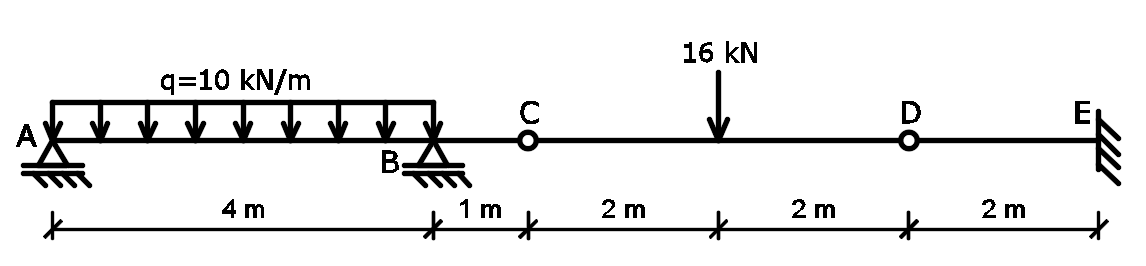
\includegraphics[width=0.85\textwidth]{pracEj1}
\end{center}
%
\noindent
Se pide:

\parte trazar los diagramas de solicitaciones (cortante y momento) de la estructura,
%
\parte dimensionar la mínima sección admisible, considerando que $b$ debe ser múltiplo de $5$ cm,
%
\parte bosquejar la deformada de la estructura y calcular los giros en los apoyos A y B, junto con el desplazamiento vertical en C, suponiendo que la rigidez flexional $EI$ es uniforme y que $E =10$ GPa.
%
\parte indicar el valor de la directa de todas las barras.




% ----------------------------
\ejercicio
%
Considere la estructura mostrada en la figura.
%
\begin{center}
	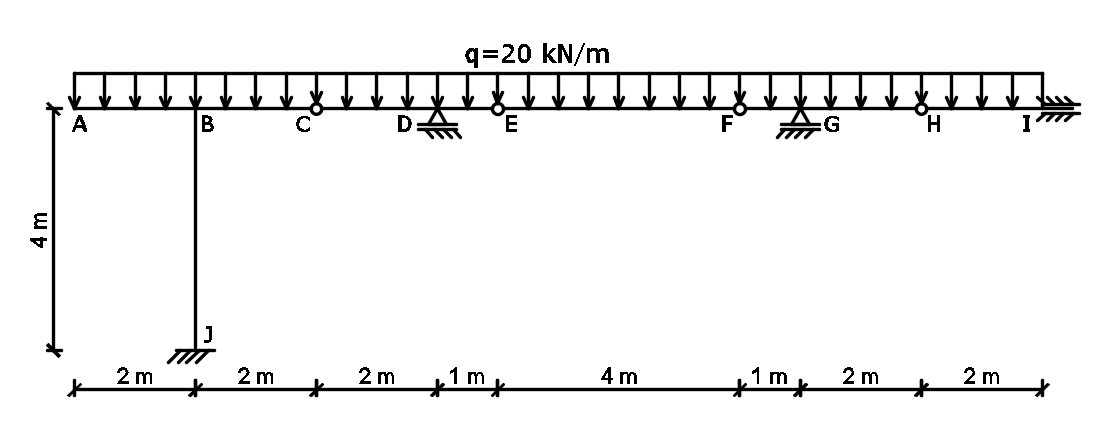
\includegraphics[width=\textwidth]{pracEj2}
\end{center}
%
\noindent
Se pide:
\parte calcular las reacciones y trazar los diagramas de solicitaciones,
\parte bosquejar la deformada de la estructura,
\parte calcular los giros sobre los apoyos y los desplazamientos de C y H en función de $EI$ (valor uniforme) y despreciando la deformación por directa.


% ----------------------------
\ejercicio
%
Considere la estructura mostrada en la figura.
%
\begin{center}
	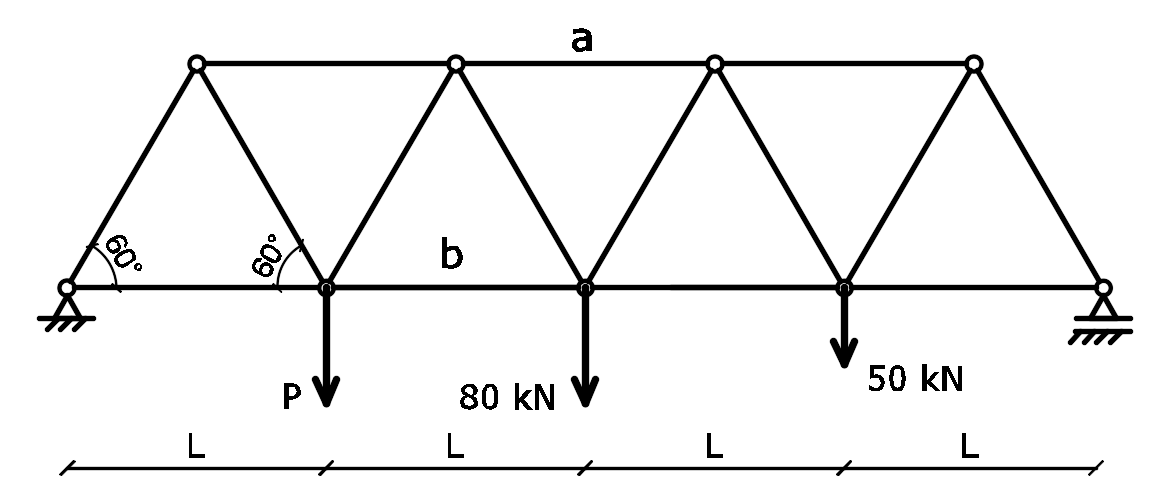
\includegraphics[width=0.82\textwidth]{pracEj3}
\end{center}
%
\noindent
Se pide:
\parte obtener analíticamente los valores de la carga $P$ para los cuales las directas en las barras $a$ y $b$ son iguales en módulo,
%
\parte verificar el resultado de la parte anterior utilizando alguna herramienta informática,
%
\parte para el valor de $P$ positivo obtenido en la parte a), dimensionar una sección transversal formada por 2 perfiles PNC a colocar en todas las barras de la estructura por igual, considerando que $\sigma_{adm} =140$ MPa.
%


\ejercicio
%
Considere la estructura mostrada en la figura, donde la carga dibujada con un círculo representa una carga movil unitaria.
%
\begin{center}
	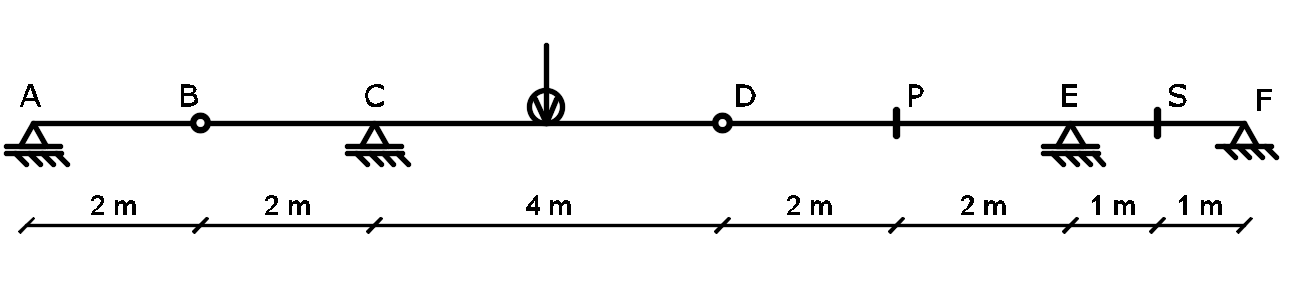
\includegraphics[width=\textwidth]{pracEj4}
\end{center}
%
\noindent
Se pide:
\parte dibujar las líneas de influencia de la reacción en el apoyo C, del cortante en P y del momento flector en S para la estructura,
\parte observando los diagramas obtenidos, indicar que ubicaciones de cargas uniformes $q=20$ kN/m provocarían máximas y mínimas RC, VP y MS.
%



\ejercicio
Considere la estructura mostrada en la figura, en la cual se tiene $EI$ uniforme.
%
\begin{center}
	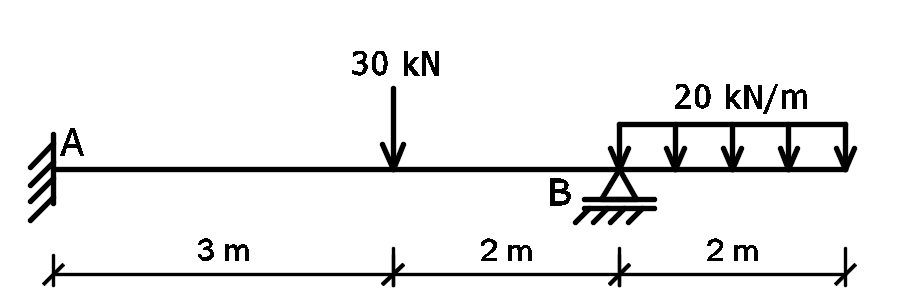
\includegraphics[width=0.65\textwidth]{pracEj5}
\end{center}
%
\noindent
Se pide:
\parte calcular las reacciones y trazar diagramas de solicitaciones aplicando el método de las ecuaciones angulares, 
\parte verificar el resultado de la parte a) utilizando alguna herramienta informática.

